%Copyright 2014 Jean-Philippe Eisenbarth
%This program is free software: you can 
%redistribute it and/or modify it under the terms of the GNU General Public 
%License as published by the Free Software Foundation, either version 3 of the 
%License, or (at your option) any later version.
%This program is distributed in the hope that it will be useful,but WITHOUT ANY 
%WARRANTY; without even the implied warranty of MERCHANTABILITY or FITNESS FOR A 
%PARTICULAR PURPOSE. See the GNU General Public License for more details.
%You should have received a copy of the GNU General Public License along with 
%this program.  If not, see <http://www.gnu.org/licenses/>.

%Based on the code of Yiannis Lazarides
%http://tex.stackexchange.com/questions/42602/software-requirements-specification-with-latex
%http://tex.stackexchange.com/users/963/yiannis-lazarides
%Also based on the template of Karl E. Wiegers
%http://www.se.rit.edu/~emad/teaching/slides/srs_template_sep14.pdf
%http://karlwiegers.com
\documentclass{scrreprt}
\usepackage{graphicx}
\graphicspath{ {./img/} }
\usepackage[outdir=./]{epstopdf}

\usepackage{listings}
\usepackage{underscore}
\usepackage[bookmarks=true]{hyperref}
\usepackage[utf8]{inputenc}
\usepackage[english]{babel}
\usepackage{amsmath,amssymb,amsthm,amsfonts}
\usepackage{xcolor}
\usepackage[acronym, toc]{glossaries}
\hypersetup{
    bookmarks=false,    % show bookmarks bar?
    pdftitle={Software Requirement Specification},    % title
    pdfauthor={Jean-Philippe Eisenbarth},                     % author
    pdfsubject={TeX and LaTeX},                        % subject of the document
    pdfkeywords={TeX, LaTeX, graphics, images}, % list of keywords
    colorlinks=true,       % false: boxed links; true: colored links
    linkcolor=blue,       % color of internal links
    citecolor=black,       % color of links to bibliography
    filecolor=black,        % color of file links
    urlcolor=purple,        % color of external links
    linktoc=page            % only page is linked
}%
\def\myversion{1.0 }
\date{}
%\title
\usepackage{hyperref}

\makenoidxglossaries

\newglossaryentry{latex}
{
    name=latex,
    description={Is a mark up language specially suited 
    for scientific documents}
}

\newglossaryentry{maths}
{
    name=mathematics,
    description={Mathematics is what mathematicians do}
}

\newacronym{api}{API}{Application Programming Interface}

\newacronym{csaf}{CSAF}{Control System Analysis Framework}

\newacronym{lec}{LEC}{Learning Enabled Controller}

\newacronym{edsl}{eDSL}{Embedded Domain Specific Language}

\newacronym{aa}{AA}{Assured Autonomy}

\newacronym{ieee}{IEEE}{Institute of Electrical and Electronics Engineers}

\newacronym{ode}{ODE}{Ordinary Differential Equation}

\newacronym{ros}{ROS}{Robot Operating System}

\newacronym{gcas}{GCAS}{Ground Collision Avoidance System}

\begin{document}

\begin{flushright}
    \rule{16cm}{5pt}\vskip1cm
    \begin{bfseries}
        \Huge{SOFTWARE REQUIREMENTS\\ SPECIFICATION}\\
        \vspace{1.9cm}
        for\\
        \vspace{1.9cm}
        Control System Analysis Framework (CSAF)\\
        \vspace{1.9cm}
        \LARGE{Version \myversion}\\
        \vspace{1.9cm}
        %Prepared by Ethan Lew\\
        \vspace{1.9cm}
        %$<$Organization$>$\\
        \vspace{1.9cm}
        \today\\
    \end{bfseries}
\end{flushright}

\tableofcontents


\chapter*{Revision History}

DISCLAIMER: This is a rough draft. The document contains many errors, and the architecture is subject to change.

%\begin{center}
%    \begin{tabular}{|c|c|c|c|}
%        \hline
%	    Name & Date & Reason For Changes & Version\\
%        \hline
%	    21 & 22 & 23 & 24\\
%        \hline
%	    31 & 32 & 33 & 34\\
%        \hline
%    \end{tabular}
%\end{center}

\chapter{Introduction}

\section{Purpose}
\acrshort{csaf} is a middleware environment for describing, simulating, and analyzing closed loop dynamical 
systems. A \acrshort{csaf} component's primary interface is \acrlong{0mq} subscribe and publish system 
components, which communicate input/output of a lump abstracted component as \acrshort{ros}msgs. It 
allows component creation using common system representations, especially for specifying controllers. The 
architecture is supportive of systems to be simulated with diverse components, agnostic to the languages 
and platforms from which they were implemented.


\section{Document Conventions}

Being middleware, the interfaces are described in the serialization formats. The features 
relate to integration tasks that are likely to be employed by the user. \\

Figures are linked in blue to their corresponding content. Acronyms are documented and linked to a glossary 
at the end of the document, labeled in blue. Hyperlinks are labeled in purple. \\

Code snippets, pseudocode and message are written in fixed width font. See Figure \ref{code:example} for 
example.

\begin{figure}[h]
\centering
\begin{lstlisting}[language=Python]
"""Example Code Snippet
"""
def main():
	return 0
\end{lstlisting}
\caption{Example Code Snippet}
\label{code:example}
\end{figure}

Math expressions are used throughout the document. They float as equations, and can be referenced. See 
Equation \ref{equ:fourier} for example.

\begin{equation} \label{equ:fourier}
\mathcal{F}_t\{g\}(f) = \int_{-\infty}^{\infty} \exp\left({-i 2\pi f t}\right) g(t) dt \\
\end{equation}


\section{Intended Audience and Reading Suggestions}

This document is designed for planning \acrshort{csaf} features and its use in the \acrlong{aa} project. 
Relevant team members are intended to read, review, and request changes to the planned architecture and 
scope. The material is intended to benefit the \acrshort{csaf} contributors and control designers using the 
project for the \acrlong{aa} project, who will use the components, interfaces and components.\\

\section{Project Scope}
Its primary use is modeling systems that utilize shields with learning enable controllers (\acrshort{lec}s). 
\acrshort{csaf} subsystems accommodate a variety of controller representation; for example, some analyses 
require explicit knowledge of the fuzzy inference being used. Rather than treating everything a black box, 
there is value in knowing whether a controller utilizes a linear control law, is produced from a network 
architecture, and so on.\\

Another use of \acrshort{csaf} is in multi-loop systems, where the control vector gets transformed before 
entering a plant. For the \acrlong{gcas} challenge problem being considered, this separates problems of 
maneuverability and attitude control. Because of this, exogenic and environmental description is pertinent. 
Path planning, collision avoidance and environmental sensing are all areas that \acrshort{csaf} will handle.\\

Some of the system description might be done in the \acrshort{edsl} CoPilot 3, which outputs a monitor 
existing as a shared object library. As such, some of the components might be present only as binaries, which 
are utilized for monitoring/controlling. Further, the platform is for projects where controllers are 
delivered by other projects, and so agnosticism to language/library/platform exists. 

\section{References}

This document uses the \acrshort{ieee} 830 SRS standard, using a \href{https://github.com/jpeisenbarth/SRS-Tex}{\LaTeX{} template} provided on GitHub.  \\


\chapter{Overall Description}

\section{Product Perspective}

CSAF serves the role of a middleware to create closed loop system simulations. A user starts with a model that they have for a dynamical system, with well-defined input, outputs and states. Shown in Figure \ref{fig:ccomp}, they will proceed to create a CSAF compatible component. The package comes with an API to make common system descriptions easy to implement, and has a wrappers if the system is more of a black box. The outcome is a system that has a subscriber to collect input and a publisher to broadcast output. \\

\begin{figure}
\centering
\includegraphics[width=0.9\textwidth]{componentcomposition.pdf}
\caption{Structure of a CSAF Compatible Component}
\label{fig:ccomp}
\end{figure}

A CSAF component is intended to represent a plant or a controller, but not closed loop system. These components can be composed together to create a closed loop dynamical system. Figure \ref{fig:csys} shows the blocks composed under a system analyzer. In the scope of controls research, this is the benefit of CSAF. Analyses can be created and performed on the modular CSAF components. \\

\begin{figure}
\centering
\includegraphics[width=0.9\textwidth]{systemanalysis.pdf}
\caption{Analyzer for Closed Loop System of CSAF Components }
\label{fig:csys}
\end{figure}


\section{Product Functions}

A user is able to

\begin{enumerate}
\item add model specifics of a dynamical system to create a compatible component
\item compose controllers together to make closed loop systems
\item simulate a closed loop systems efficiently
\item design custom analyses, and is supported with libraries and documentation
\end{enumerate}

Figure \ref{fig:uworkflow} shows the user workflow for a systems analysis, from start to finish. All blocks in the control diagram must exist as components. Then, the components are composed together to achieve the controlled system. The system is ready to be simulated or analyzed.

\begin{figure}
\centering
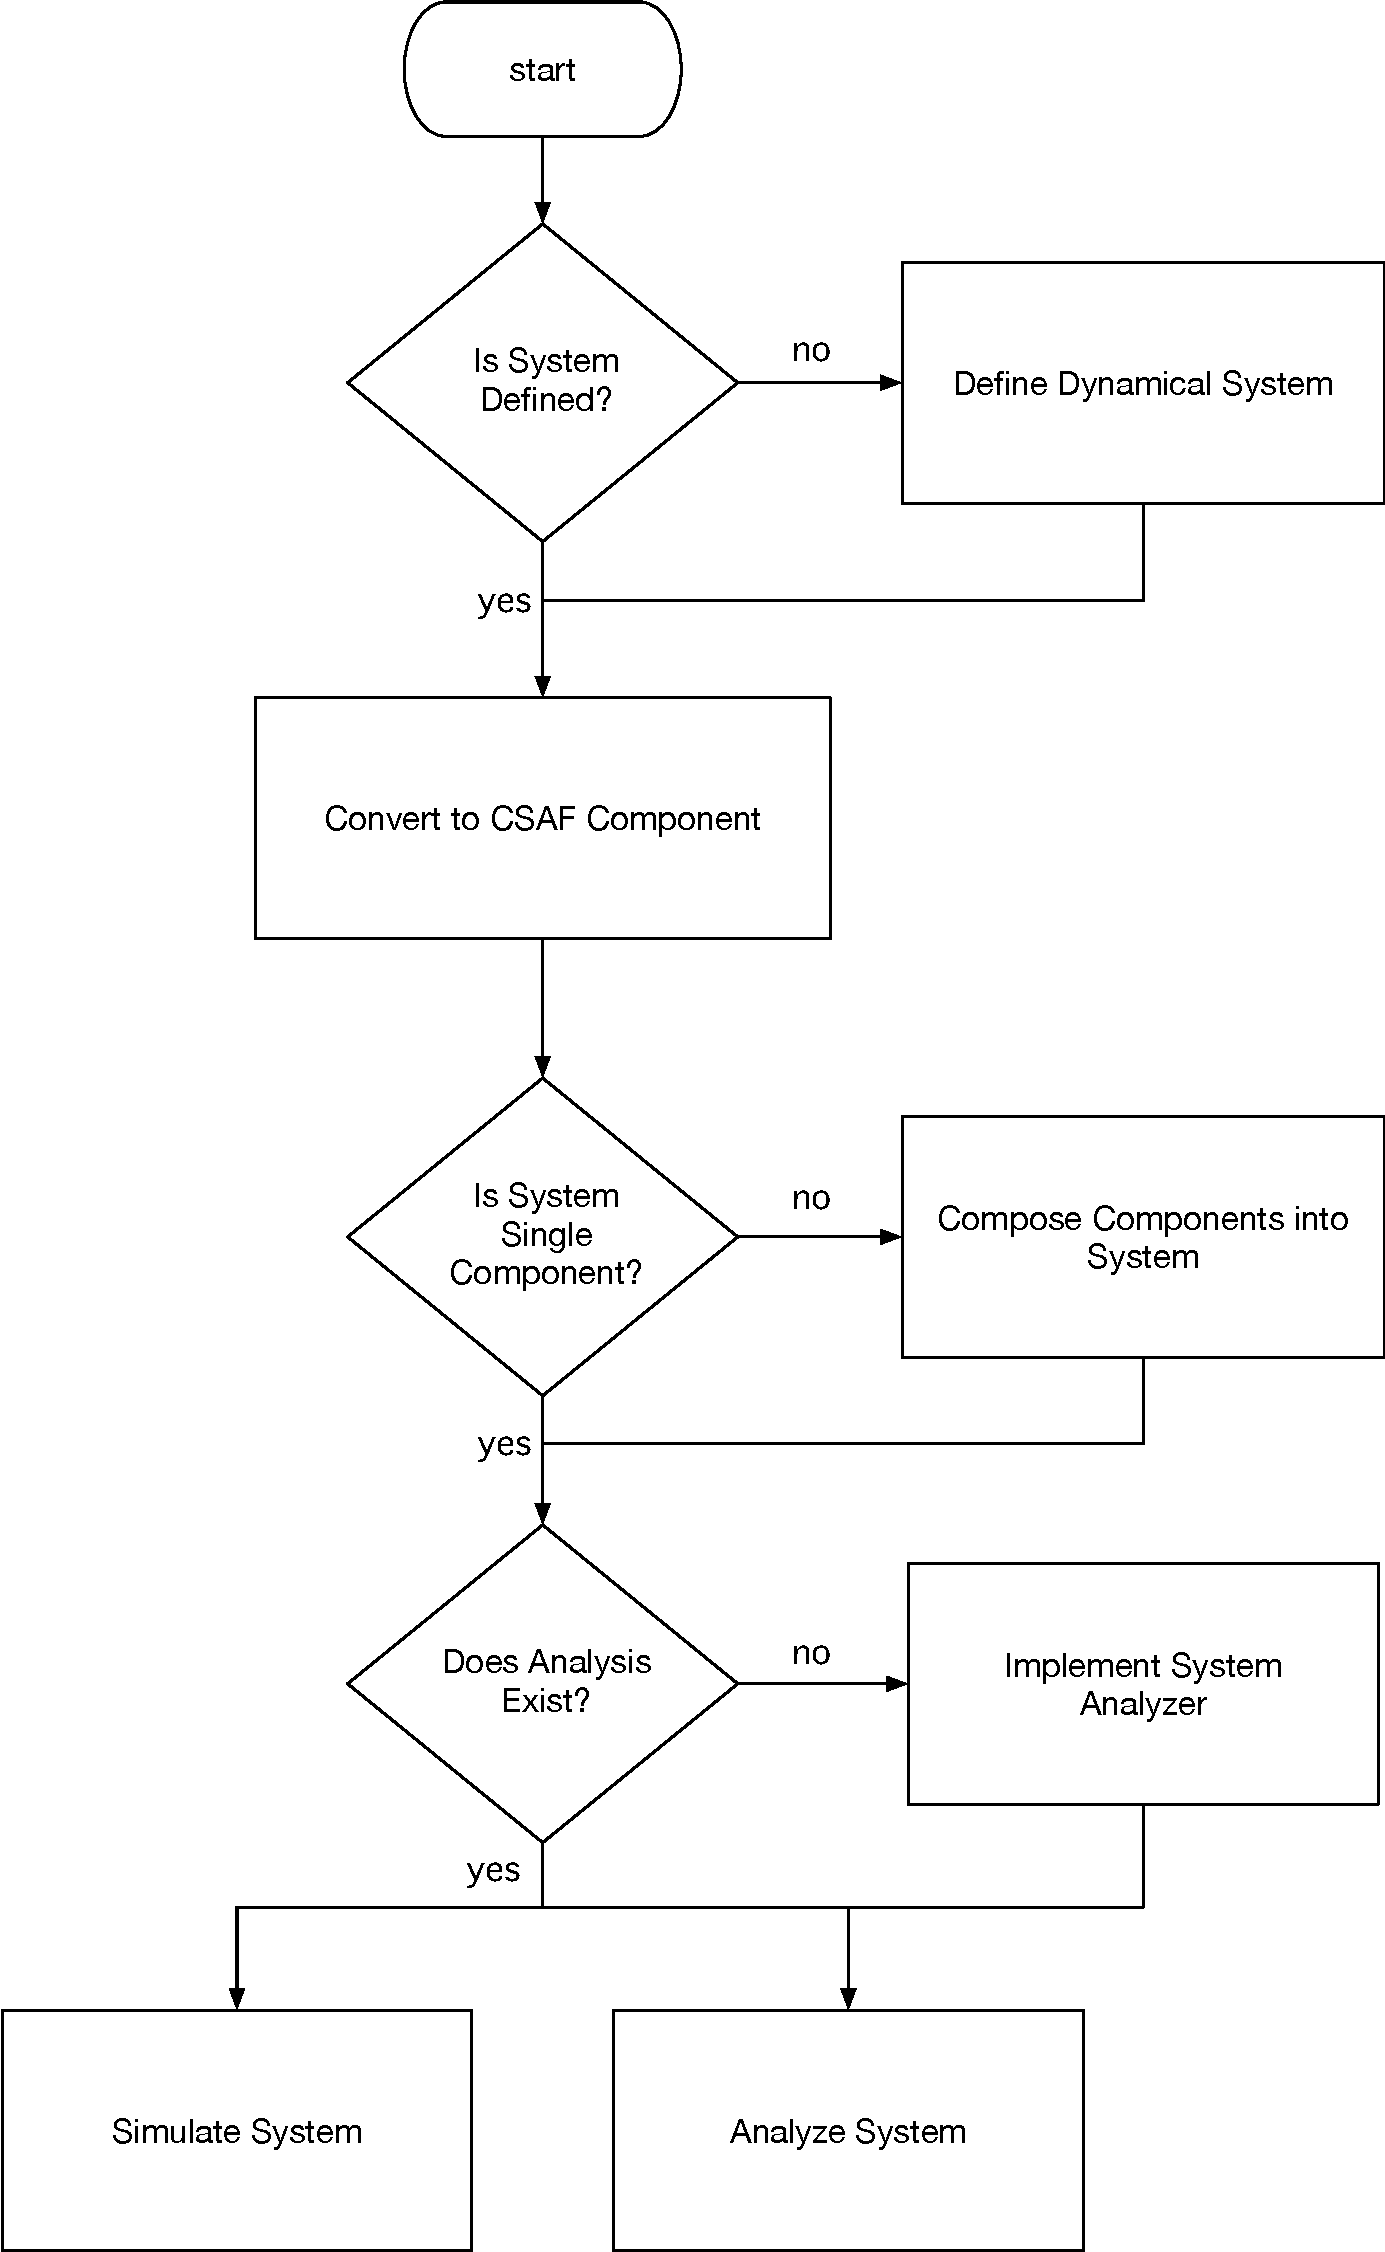
\includegraphics[width=0.85\textwidth]{userworkflow2.pdf}
\caption{ CSAF System Analysis User Workflow }
\label{fig:uworkflow}
\end{figure}

\section{User Classes and Characteristics}

CSAF's user workflow is restricted to software developers, systems engineers and researchers. The users implementing components are required to have substantial knowledge of programming and system theory. The workflow output is to provide results for a controls research project. As such, secondary users are project managers and reviewers. 


\section{Operating Environment}

CSAF is implemented in modern python (3.5+), with specific packages for numerical/controls computing. Also, it has optional package requirements, like tensorflow and RosPy needed for specific features. Its primary use is to operate inside a debian based docker container for its delivery in the Assured Autonomy project. For full use, it will require a OS with CoPilot installed, needing Haskell and C toolchains.  

\section{Design and Implementation Constraints}
$<$Describe any items or issues that will limit the options available to the 
developers. These might include: corporate or regulatory policies; hardware 
limitations (timing requirements, memory requirements); interfaces to other 
applications; specific technologies, tools, and databases to be used; parallel 
operations; language requirements; communications protocols; security 
considerations; design conventions or programming standards (for example, if the 
customer’s organization will be responsible for maintaining the delivered 
software).$>$

\section{User Documentation}

As CSAF users will need detailed knowledge of its architecture and API to use it effectively, documentation is important. Its code repository contain a number of markdown files that outline the installation and setup. For object and function level documentation, the code uses an ample amount of Python docstrings, which can be used to autogenerate API documentation if the code comments are suitably detailed. \\

API level documentation is not enough, and  a user manual is available. This manual is conscience of task oriented documentation; the workflow is discussed and examples are provided for intended implementation use. Further, the use cases are also described in Jupyter notebooks, which provide an interactive platform to experiment with code.

\section{Assumptions and Dependencies}

$<$List any assumed factors (as opposed to known facts) that could affect the 
requirements stated in the SRS. These could include third-party or commercial 
components that you plan to use, issues around the development or operating 
environment, or constraints. The project could be affected if these assumptions 
are incorrect, are not shared, or change. Also identify any dependencies the 
project has on external factors, such as software components that you intend to 
reuse from another project, unless they are already documented elsewhere (for 
example, in the vision and scope document or the project plan).$>$


\chapter{External Interface Requirements}

\section{User Interfaces}
$<$Describe the logical characteristics of each interface between the software 
product and the users. This may include sample screen images, any GUI standards 
or product family style guides that are to be followed, screen layout 
constraints, standard buttons and functions (e.g., help) that will appear on 
every screen, keyboard shortcuts, error message display standards, and so on.  
Define the software components for which a user interface is needed. Details of 
the user interface design should be documented in a separate user interface 
specification.$>$

\section{Hardware Interfaces}
$<$Describe the logical and physical characteristics of each interface between 
the software product and the hardware components of the system. This may include 
the supported device types, the nature of the data and control interactions 
between the software and the hardware, and communication protocols to be 
used.$>$

\section{Software Interfaces}
$<$Describe the connections between this product and other specific software 
components (name and version), including databases, operating systems, tools, 
libraries, and integrated commercial components. Identify the data items or 
messages coming into the system and going out and describe the purpose of each.  
Describe the services needed and the nature of communications. Refer to 
documents that describe detailed application programming interface protocols.  
Identify data that will be shared across software components. If the data 
sharing mechanism must be implemented in a specific way (for example, use of a 
global data area in a multitasking operating system), specify this as an 
implementation constraint.$>$

\section{Communications Interfaces}
$<$Describe the requirements associated with any communications functions 
required by this product, including e-mail, web browser, network server 
communications protocols, electronic forms, and so on. Define any pertinent 
message formatting. Identify any communication standards that will be used, such 
as FTP or HTTP. Specify any communication security or encryption issues, data 
transfer rates, and synchronization mechanisms.$>$


%\chapter{System Features}
This section organizes the functional requirements for \acrshort{csaf} . As the package serves as a library and middleware, it is organized by tasks commonly needed for system analysis.

\section{[\acrshort{csaf} -01] Component Creation}
The user is able to take common model description and put them into the \acrshort{csaf}  environment.

\subsection{Description and Priority}
This is a high priority feature. For now, emphasis is put on the integration of a F16 model and possibly other aerodynamic models. Also, a variety of controllers need to be converted to this middleware.

\subsection{Stimulus/Response Sequences}
The user
\begin{enumerate}
\item identifies their model to a common model description (dynamical, linear, fuzzy, neural, etc)
\item wraps their model to interfaces required by the \acrshort{csaf}  middleware
\item tests the new component on the \acrshort{csaf}  platform
\end{enumerate}

\subsection{Functional Requirements}
\begin{enumerate}
\item REQ-1 \quad the user can transform a system written in python into a \acrshort{csaf}  component
\end{enumerate}

\section{[\acrshort{csaf} -02] Time Domain Simulation}
The user is able to take a \acrshort{csaf}  system and simulate it.

\subsection{Description and Priority}
This is a high priority feature.

\subsection{Stimulus/Response Sequences}
The user
\begin{enumerate}
\item has a valid system of components
\item specifies initial states for all components
\item specifies a time interval AND valid conditions for the system
\item run a simulator, and gets a time trace as an output
\end{enumerate}

\subsection{Functional Requirements}
\begin{enumerate}
\item REQ-1 \quad the user receives a time trace as an output
\item REQ-2 \quad the user can view the system changing in a real-time dashboard
\end{enumerate}


\section{[\acrshort{csaf} -03] Component Composition}
The user is able to compose components to create a controlled plant system.

\subsection{Description and Priority}
This is a high priority feature.

\subsection{Stimulus/Response Sequences}
The user
\begin{enumerate}
\item specifies input and output signal between components
\item checks that they have valid topology using a checker
\end{enumerate}

\subsection{Functional Requirements}
\begin{enumerate}
\item REQ-1 \quad the user can specify inner/outer loop systems
\item REQ-2 \quad a checker ensures that the components are correct configured before further use
\end{enumerate}

\section{[\acrshort{csaf} -04] CoPilot Support}
The user is able to add CoPilot monitors to their systems.

\subsection{Description and Priority}
This is a high priority feature.

\subsection{Stimulus/Response Sequences}


\subsection{Functional Requirements}

\section{[\acrshort{csaf} -05] Controller Monitoring and Shields}

\subsection{Description and Priority}
This is a high priority feature.

\subsection{Stimulus/Response Sequences}


\subsection{Functional Requirements}

\section{[\acrshort{csaf} -06] Fuzzy Controller Representation}

\subsection{Description and Priority}
This is a medium priority feature.

\subsection{Stimulus/Response Sequences}


\subsection{Functional Requirements}

\section{[\acrshort{csaf} -07] Neural Controller Representation}

\subsection{Description and Priority}
This is a medium priority feature.

\subsection{Stimulus/Response Sequences}


\subsection{Functional Requirements}

\section{[\acrshort{csaf} -08] Time Traces}

\subsection{Description and Priority}
This is a medium priority feature.

\subsection{Stimulus/Response Sequences}


\subsection{Functional Requirements}


%\section{System Feature 2 (and so on)}
%
%
%\chapter{Other Nonfunctional Requirements}
%
%\section{Performance Requirements}
%$<$If there are performance requirements for the product under various 
%circumstances, state them here and explain their rationale, to help the 
%developers understand the intent and make suitable design choices. Specify the 
%timing relationships for real time systems. Make such requirements as specific 
%as possible. You may need to state performance requirements for individual 
%functional requirements or features.$>$
%
%\section{Safety Requirements}
%$<$Specify those requirements that are concerned with possible loss, damage, or 
%harm that could result from the use of the product. Define any safeguards or 
%actions that must be taken, as well as actions that must be prevented. Refer to 
%any external policies or regulations that state safety issues that affect the 
%product’s design or use. Define any safety certifications that must be 
%satisfied.$>$
%
%\section{Security Requirements}
%$<$Specify any requirements regarding security or privacy issues surrounding use 
%of the product or protection of the data used or created by the product. Define 
%any user identity authentication requirements. Refer to any external policies or 
%regulations containing security issues that affect the product. Define any 
%security or privacy certifications that must be satisfied.$>$
%
%\section{Software Quality Attributes}
%$<$Specify any additional quality characteristics for the product that will be 
%important to either the customers or the developers. Some to consider are: 
%adaptability, availability, correctness, flexibility, interoperability, 
%maintainability, portability, reliability, reusability, robustness, testability, 
%and usability. Write these to be specific, quantitative, and verifiable when 
%possible. At the least, clarify the relative preferences for various attributes, 
%such as ease of use over ease of learning.$>$
%
%\section{Business Rules}
%$<$List any operating principles about the product, such as which individuals or 
%roles can perform which functions under specific circumstances. These are not 
%functional requirements in themselves, but they may imply certain functional 
%requirements to enforce the rules.$>$
%
%
%\chapter{Other Requirements}
%$<$Define any other requirements not covered elsewhere in the SRS. This might 
%include database requirements, internationalization requirements, legal 
%requirements, reuse objectives for the project, and so on. Add any new sections 
%that are pertinent to the project.$>$
%
%\section{Appendix A: Glossary}
%%see https://en.wikibooks.org/wiki/LaTeX/Glossary
%$<$Define all the terms necessary to properly interpret the SRS, including 
%acronyms and abbreviations. You may wish to build a separate glossary that spans 
%multiple projects or the entire organization, and just include terms specific to 
%a single project in each SRS.$>$
%
%\section{Appendix B: Analysis Models}
%$<$Optionally, include any pertinent analysis models, such as data flow 
%diagrams, class diagrams, state-transition diagrams, or entity-relationship 
%diagrams.$>$
%
%\section{Appendix C: To Be Determined List}
%$<$Collect a numbered list of the TBD (to be determined) references that remain 
%in the SRS so they can be tracked to closure.$>$


\printnoidxglossary[type=\acronymtype]

\end{document}
